\chapter{Limiti e continuità}

\section{Limiti di funzioni}
I limiti delle funzioni sono utili per capire il comportamtento di una funzione vicino ad un determinato punto.

\begin{figure}[ht]
    \centering
    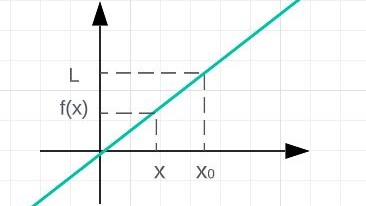
\includegraphics[width = 7cm]{images/limiti1.JPG}
\end{figure}

Presa una funzione $f:A\subset\mathbb{R}\rightarrow\mathbb{R}$, vogliamo tradurre in linguaggio matematico che la funzione si avvicina ad un valore $l$ quando $x$ si avvicina ad $x_0$.

\subsection*{Limiti $x\to x_0$}

\begin{definition}[Limite]
    Dato $f:A\rightarrow\mathbb{R}, x_0\in\mathbb{R}$ diciamo che $f(x)\rightarrow l$ per $x\rightarrow x_0$ e scriviamo:
    \begin{equation}\label{eq:limite_def}
        \lim_{x\to x_0}f(x)=l
    \end{equation}
    $\text{Se } \forall\varepsilon>0, \exists\delta>0:|f(x)-l|<\varepsilon,\forall x\in A:0<|x-x_0|<\delta \text{ con } x\neq x_0$
\end{definition}

Quindi presa una qualsiasi funzione e raffigurata su un piano cartesiano, stando alla formula \ref{eq:limite_def}, dobbiamo trovare $l\pm\varepsilon$ e $x_0\pm\delta$, che ci permettano di determinare la regione della nostra funzione.

\begin{figure}[ht]
    \centering
    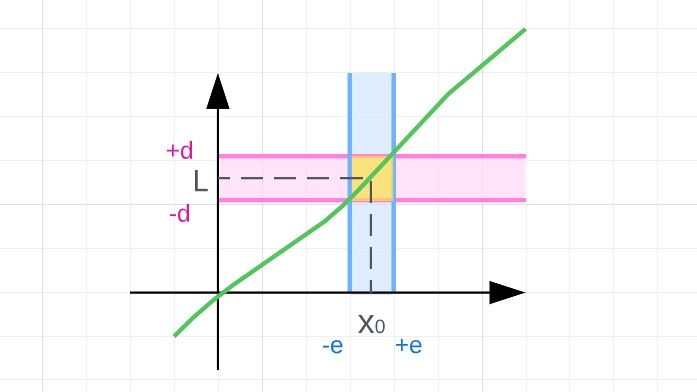
\includegraphics[width = 11cm]{images/limiti2.JPG}
    \caption{Limite per $x\rightarrow 0$}
    \label{fig:limite_xto0}
\end{figure}

Tutto ciò risulta facile con i numeri finiti ma come faccio a trovare matematicamente numeri molto piccoli nel caso in cui la mia funzione tende a $\pm\infty$?

\begin{definition}[Limiti di infinito]
Data $f:A\subset\mathbb{R}\rightarrow\mathbb{R}, x_0\in\mathbb{R}$ diciamo che $f(x)\rightarrow -\infty(+\infty)$ per $x\rightarrow x_0$ e scriviamo:
\begin{equation}
    \lim_{x\to x_0}f(x)=-\infty(+\infty)
\end{equation}
 $\text{Se } \forall M\in\mathbb{R},\exists\delta>0:f(x)<M(f(x)>M),\forall x\in A:0<|x-x_0|<\delta$

\begin{figure}[ht]
    \centering
    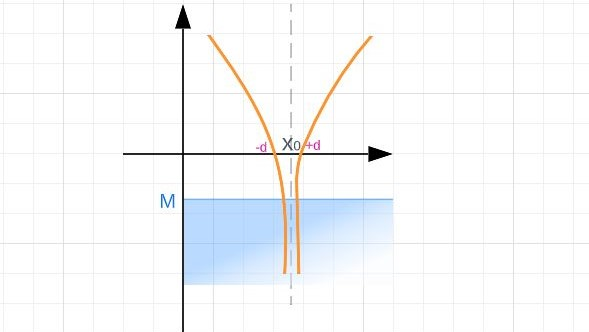
\includegraphics[width = 10cm]{images/limiti3.JPG}
    \caption{Limite che tende a $-\infty$}
    \label{fig:limite3}
\end{figure}
\end{definition}


\begin{example}
    $\lim_{x\to x_0}\ln x=-\infty$
    
    Fissiamo $M\in\mathbb{R}$. Volendo ottenere $\ln x<M$, procediamo tramite l'esponenziale: $e^{\ln x}<e^M\rightarrow x<e^M=\delta$.
    
    Quindi per $x$ che $\in$ dominio $\ln$ t.c. $0<|x-0|<e^M$ ovvero $0<x<e^M$ vale $f(x)<M$.
\end{example}

Come si sa, risolto un problema nè nasce un altro: come si esprime matematicamente il concetto di $\lim_{x\to\pm\infty}f(x)=0$?

\subsection*{Limiti $x\to\infty$}
\begin{definition}[Limiti che tendono a infinito]
Data $f:A\subset\mathbb{R}\rightarrow\mathbb{R}$ dico che:
\begin{equation}
    \lim_{x\to+\infty}f(x)=l
\end{equation}
$\text{Se }\forall\varepsilon>0, \exists N\in\mathbb{R} \text{ t.c. } |f(x)-l|\leq\varepsilon \text{ per } x\in A \text{ t.c. } x>N$

\begin{figure}[ht]
    \centering
    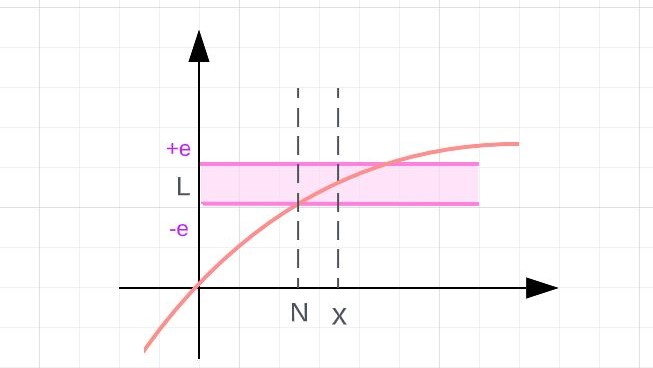
\includegraphics[width = 10cm]{images/limiti4.JPG}
    \caption{$\lim{x\to+\infty}$}
    \label{fig:limite_infinito}
\end{figure}

La stessa cosa vale a $-\infty$ ma $x$ deve essere $<N$.
\end{definition}

Con queste definizioni possiamo verificare i limiti più comuni:
\begin{itemize}
    \item $\lim_{x\to+\infty}e^x=+\infty$
    \item $\lim_{x\to-\infty}e^x=0$
    \item $\lim_{x\to+\infty}a^x=0$
    \item $\lim_{x\to-\infty}a^x=+\infty$
    \item $\lim_{x\to+\infty}\log_ax=\begin{cases}+\infty \text{ se } a>1\\-\infty \text{ se } 0<a<1\end{cases}$
    \item $\lim_{x\to0}\log_ax=\begin{cases}-\infty \text{ se } a>1\\+\infty \text{ se } 0<a<1\end{cases}$
    \item $\lim_{x\to+\infty}x^\alpha=\begin{cases}+\infty \text{ se } \alpha>0\\1 \text{ se } \alpha =0\\0 \text{ se } \alpha <0\end{cases}$
\end{itemize}

\begin{osservation}
    Nella maggior parte dei casi se $x_0\in$ dominio di $f$ allora $\lim_{x\to x_0}f(x)=f(x_0)$.
\end{osservation}

\subsection*{Limiti destri e sinistri}
Presa una funzione come $f(x)=\frac{1}{x}$

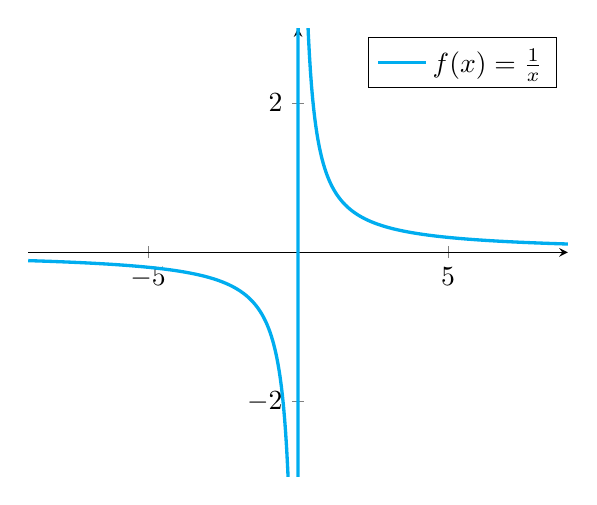
\begin{tikzpicture}
    \begin{axis}[xmin=-9,xmax=9,ymin=-3,ymax=3,
    axis x line=middle,
    axis y line=middle]
    \addplot [very thick, domain=-9:9, samples=500, color=cyan,]{1/x};\addlegendentry{\(f(x)=\frac{1}{x}\)}
    \end{axis}
\end{tikzpicture}

notiamo come per $x\rightarrow 0$ troviamo un duplice andamento. Se ci spostiamo verso destra la funzione sembra tendere a $+\infty$, al contrario, verso sinistra, a $-\infty$. Diremo quindi che $\lim_{x\to 0^+}\frac{1}{x}=+\infty$ e $\lim_{x\to 0^-}\frac{1}{x}=-\infty$.

\begin{definition}[Limiti destri e sinistri]
    Dando una definizione possiamo dire che:
    \begin{equation}
        \lim_{x\rightarrow x_0^+}f(x)=l
    \end{equation}
    $\text{Se } \forall x>0, \exists\delta>0:|f(x)-l|<\varepsilon \text{ per } x\in A \text{ con } x_0<x<x_0+\delta$.
    
    Lo stesso vale per il $\lim_{x\rightarrow x_0^-}f(x)=l \text{ con } x_0-\delta<x<x_0$.
\end{definition}


\subsection{Operazioni tra limiti}
Guardiamo ora le operazioni tra i limiti.

\begin{thm}
    Siano $f_1, f_2:A\subset\mathbb{R}\rightarrow\mathbb{R}$ e sia 
    \begin{equation}
        l_i=\lim_{x\to x_0}f_i(x) \text{ con } i=1,2 
    \end{equation}
    $x_0\in\overline{\mathbb{R}}=\mathbb{R}\cap\{\-\infty,+\infty\}, l_1, l_2\in\mathbb{R}$.
\end{thm}

\begin{definition}[Somma]\label{lim:th:somma}
    \begin{equation*}
        \lim_{x\to x_0}f_1(x)+f_2(x)=l_1+l_2    
    \end{equation*}
    La somma dei limiti è uguale al limite della somma.
\end{definition}

\begin{definition}[Prodotto]\label{lim:th:prodotto}
    \begin{equation*}
        \lim_{x\to x_0}f_1(x)*f_2(x)=l_1*l_2    
    \end{equation*}
    Il prodotto dei limiti è uguale al limite del prodotto.
\end{definition}

\begin{definition}[Quoziente]
    \begin{equation*}
        \lim_{x\to x_0}\frac{f_1(x)}{f_2(x)}=\frac{l_1}{l_2} \text{ se } l_2\neq 0
    \end{equation*}
    Il quoziente dei limiti è uguale al limite del quoziente con il denominatore diverso da 0.
\end{definition}

\begin{example}
    $\lim_{x\to x_0}x^2=$\\$\lim_{x\to x_0}x*x$\\Per il Teorema del prodotto \ref{lim:th:prodotto} il $\lim_{x\to x_0}x^2=x_0*x_0=x_0^2$.
    
    La stessa cosa vale per il limite di $x^3$.
    Quindi in generale possiamo dire che $\lim_{x\to x_0}ax^n=\lim_{x\to x_0}a*\lim_{x\to x_0}x^n=ax_0^n$.
\end{example}


\section{Limiti di polinomi}
Se fino ad ora avete visto i limiti solo come delle semplici relazioni, aspettate a dirlo prima di leggere i paragrafi successivi. In questa sezione, infatti, cercheremo di calcolare i risultati di limiti più complessi.

Dato il polinomio $P(x)=\sum_{i=0}^{n}ax^i=a^nx^n+...+a_0$, per il Teorema della somma \ref{lim:th:somma} abbiamo che:
\begin{equation}
    \lim_{x\to x_0}P(x)=\sum_{i=0}^{n}\lim_{x\to x_0}a_in^i=\sum_{i=0}^{n}a_ix_0^i=P(x_0)
\end{equation}
Ciò che abbiamo fatto è stato semplicemente sostituire il termine $x_0$ al posto della $x$.

\subsection*{Polinomi per $x\to\pm\infty$}\label{subsec:polinf}
Applichiamo quanto appreso per calcolare i limiti dei polinomi per $x\to\pm\infty$.

Se ad esempio prediamo il $\lim_{x\to+\infty}2x^3-x^2+1$ questo è uguale a $+\infty -\infty$ ma non può essere perchè è una forma indeterminata.
Questo accade perchè la forma risolutiva di questi limiti è diversa rispetto a quelli precedenti (non basta sostituire $x$ con $\pm\infty$).

Quindi per risolvere questo limite dobbiamo raccogliere il termine maggiore e dividere i restanti per quel termine:
\begin{equation*}
    \lim_{x\to+\infty}x^3(2-\frac{1}{x}+\frac{1}{x^3})
\end{equation*}
Ora che abbiamo trovato $f_1(x)=x^3$ e $f_2(x)=2-\frac{1}{x}+\frac{1}{x^3}$, possiamo sostituire i valori della x e otterremo $\lim_{x\to+\infty}+\infty*2$, per il Teorema della somma \ref{lim:th:somma} $=+\infty$.
    
In generale abbiamo che:
\begin{equation*}
    \lim_{x\to\pm\infty}P(x)=\lim_{x\to\pm\infty}a_nx^n+...+a_0
\end{equation*}
\begin{equation*}
    \lim_{x\to\pm\infty}x^n(a_n+\frac{a_n-1}{x}+...+\frac{a_0}{x})
\end{equation*}
Dato che tutti i termini all'interno della parentesi tendono a 0 otteniamo:
\begin{itemize}
    \item $$lim_{x\to+\infty}P(x)=
    \begin{cases}
        +\infty \text{ se } a_n>0\\
        -\infty \text{ se } a_n<0
    \end{cases} 
    $$
    \item $$lim_{x\to-\infty}P(x)=
    \begin{cases}
        +\infty \text{ se n è pari, } a_n>0 \text{ oppure } a_n \text{ dispari } a_n<0\\
        -\infty \text{ in tutti gli altri casi }
    \end{cases} 
    $$
\end{itemize}

\subsection*{Limiti di polinomi razionali}
\begin{equation}
    \lim{x\to x_0}\frac{P(x)}{Q(x)}=\frac{\lim_{x\to x_0}P(x)}{\lim_{x\to x_0}Q(x)}=\frac{P(x_0)}{Q(x_0)} \text{ per } x_0 \text{ t.c. } Q(x_0)\neq 0
\end{equation}

\begin{example}
    $\lim_{x\to 3}\frac{x^2-1}{2x+1}$\\$\lim_{x\to 3}\frac{x^2-1}{2x+1}=\frac{3^2-1}{2*3+1}=\frac{8}{7}$
\end{example}

Più difficile è sicuramente calcolare il $\lim_{x\to\pm\infty}\frac{P(x)}{Q(x)}$ con $P$ e $Q$ polinomi o anche il $\lim_{x\to+\infty}e^x+\cos x$.
Con un pò di logica possiamo risolvere il limite precedente in quanto $e^x$ per $x$ che tende a $+\infty$ va a $+\infty$ mentre il $\cos$ oscilla sempre tra -1 e 1.
Ma ciò non basta perchè dobbiamo dimostrarlo.

Un facile modo per risolvere i limiti di questo tipo è seguire questi 8 casi:

\renewcommand{\labelenumii}{\arabic{enumi}.\arabic{enumii}}
\begin{enumerate}[label=\textbf{\arabic*})]
    \item $l_1=+\infty, f(x)$ è limitata dal basso per $x$ vicino a $x_0$, ovvero $\exists m\in\mathbb{R}$ t.c. $f_2(x)\geq m$ per $x$ vicino a $x_0$.
    
    % \begin{figure}[ht]
    %     \centering
    %     \includegraphics{}
    %     \caption{Caption}
    %     \label{fig:my_label}
    % \end{figure}
    
    Dato che la somma va a $+\infty$ perchè $f_2$ è limitata dal basso e non può quindi trovarsi sotto un dato valore. Allora:
    \begin{equation}
        \lim_{x\to x_0}f_1(x)+f_2(x)=+\infty
    \end{equation}
    
    Vediamo con un esempio:
    \begin{example}
        $f_1(x)=x^2, f_2(x)=\sin x$\\$f_1(x)$ tende a $+\infty$, $f_2(x)$ è $\geq -1$ quindi $\lim_{x\to+\infty}x^2+\sin x=+\infty$.
        
        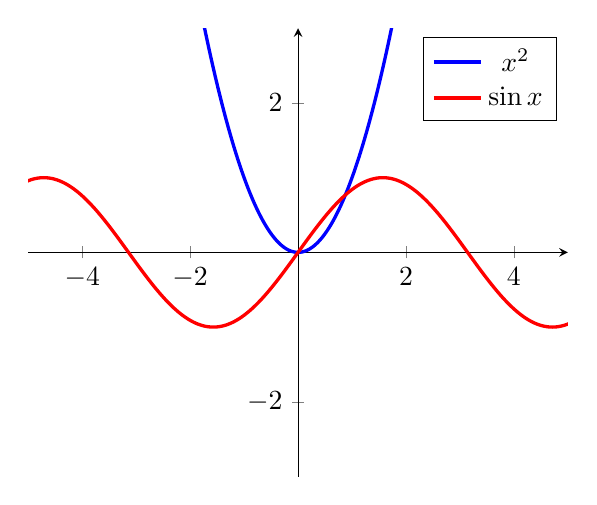
\begin{tikzpicture}
            \begin{axis}[xmin=-5,xmax=5,ymin=-3,ymax=3,
            axis x line=middle,
            axis y line=middle]
            \addplot [very thick, domain=-5:5, samples=500, color=blue,]{x^2};\addlegendentry{$x^2$}
            \addplot [very thick, domain=-10:10, samples=500, color=red,]{sin(deg(x))};\addlegendentry{$\sin x$}
            \end{axis}
        \end{tikzpicture}
        
    \end{example}
    
    Lo stesso ragionamento può essere usato con le funzioni invertite dove $l_1=-\infty$ e $f_2(x)\leq M$.
    \begin{equation}
        \lim_{x\to x_0}f_1(x)+f_2(x)=-\infty
    \end{equation}
    
    \item $l_1=l_2=\pm\infty$. Allora:
    \begin{equation}
        \lim_{x\to x:0}f_1(x)+f_2(x)=\pm\infty
    \end{equation}
    \begin{example}
        $\lim_{x\to-\infty}x^3+2x=-\infty$
    \end{example}
    
    \item $l_1=+\infty, l_2=-\infty$ in questo caso ci troviamo difronte ad una forma indeterminata, vuol dire che per ora non conosciamo ancora il risultato del limite.
    \begin{example}
        $\lim_{x\to+\infty}\ln x-x^2=$ forma indeterminata
    \end{example}
    
    \item
    \begin{enumerate}[label=\textbf{\arabic*})]
        \item $l_1=+\infty, l_2>0$. Allora:
    \begin{equation}
        \lim_{x\to x_0}f_1(x)*f_2(x)=\pm\infty
    \end{equation}
    \begin{example}
        $\lim_{x\to+\infty}e^x*\arctan x=+\infty$
    \end{example}
    
    \item $l_1=\pm\infty, l2<0$. Allora:
    \begin{equation}
        \lim_{x\to x_0}f_1(x)*f_2(x)=-(\pm\infty)
    \end{equation}
    \begin{example}
        $\lim_{x\to-\infty}e^{-x}*\arctan x=-\infty$
    \end{example}
    \end{enumerate}
    
\end{enumerate}

    
    I metodi applicati nella parte \ref{subsec:polinf}, relativa ai polinomi che tendono a $\pm\infty$, sono gli stessi per risolvere i limiti dei polinomi razionali.
    
    \begin{enumerate}[label=\textbf{\arabic*})]\setcounter{enumi}{4}
        \item $\lim_{x\to\pm\infty}\frac{P(x)}{Q(x)}$ con $Q(x)=\sum_{i=0}^{n}b_ix^i$
        \begin{equation*}
            \lim_{x\to+\infty}\frac{a_nx^n+...+a_0}{b_nx^n+...+b_0}
        \end{equation*}
        A questo punto raccolgo entrambe i polinomi:
        \begin{equation*}
            \lim_{x\to+\infty}\frac{x^n(a_n+...+\frac{a_0}{x^n})}{x^m(b_m+...+\frac{b_0}{x^m})}
        \end{equation*}
        Da ciò otteniamo:
        \begin{equation*}
            \lim_{x\to+\infty}x^{n-m}\frac{a_n}{b_m}=\begin{cases}
                0 \text{ se } n<m\\
                \frac{a_n}{b_m} \text{ se } n=m\\
                +\infty \text{ se } n>m \text{ e } \frac{a_n}{b_n}>0\\
                -\infty \text{ se } n>m \text{ e } \frac{a_n}{b_n}<0
            \end{cases}
        \end{equation*}
        \begin{center}
            oppure
        \end{center}
        \begin{equation*}
            \lim_{x\to-\infty}\frac{P(x)}{Q(x)}=\begin{cases}
                0 \text{ se } n<m\\
                \frac{a_n}{b_m} \text{ se } n=m\\
                +\infty \text{ se } n>m \text{ oppure n è pari e } \frac{a_n}{b_n}>0\\
                -\infty \text{ se } n>m \text{ oppure n è dispari e } \frac{a_n}{b_n}>0\\
                -\infty \text{ se } n>m \text{ oppure n è pari e } \frac{a_n}{b_n}<0\\
                +\infty \text{ se } n>m \text{ oppure n è dispari e } \frac{a_n}{b_n}<0\\
            \end{cases}
        \end{equation*}
        Constatato il complicato e inutile lavoro mnemonico che dovremmo effetturare per ricordare tutte queste definizioni, possiamo, molto più semplicemente, applicare il \textbf{teorema dei gradi} (vedi Sezione \ref{subsec:tdg}).
    
        \item $l_1>0, l_2=0^+$, ovvero $f_2(x)\to 0$ per $x\to x_0$ e $f_2(x)>0$ vicino a $x_0$. Allora:
        \begin{equation}
            \lim_{x\to x_0}\frac{f_1(x)}{f_2(x)}=+\infty
        \end{equation}
    
        \item $l_1=\pm\infty, l_2>0$. Allora:
        \begin{equation}
            \lim_{x\to x_0}\frac{f_1(x)}{f_2(x)}=\pm\infty
        \end{equation}
        \begin{example}
            $\lim_{x\to 0}\frac{\log_{\frac{1}{2}}x}{\cos x}=+\infty$
        \end{example}
        
        \item $l_1=\pm\infty, l_2=0^{\pm}$. Allora:
        \begin{equation}
            \lim_{x\to x_0}\frac{f_1(x)}{f_2(x)}=\pm\infty
        \end{equation}
        \begin{example}
            $\lim_{x\to 0^+}\frac{\ln x}{x}=-\infty$
        \end{example}
        
    \end{enumerate}
    

\subsection*{Altri casi}
Dato il limite $\lim_{x\to x_0}f_1(x)^{f_2(x)}$ cosa succede per $l_1=\pm\infty, l_1=0, l_2=\pm\infty, l_2=0$?

\begin{enumerate}[label=\textbf{\arabic*})]
    \item $l_1>1, l_2=+\infty$
    
    \begin{equation}
        \lim_{x\to x_0}f_1(x)^{f_2(x)}=+\infty
    \end{equation}
    La funzione $f_1$ è $>1$ e la stiamo elevando ad un numero molto grande che tende a inifinito. Il risultato sarà quindi $+\infty$. Infatti una base maggiore di 1, elevata ad un numero molto grande, produrrà a sua volta un numero elevato.
    \begin{example}
        $\lim_{x\to x_0}\arctan x^{2+\ln x}=+\infty$
    \end{example}
    
    \item $l_1>1, l_2=-\infty$
    
    \begin{equation}
        \lim_{x\to x_0}f_1(x)^{f_2(x)}=0
    \end{equation}
    
    Questo perchè secondo il ragionamento del caso precedente, un numero maggiore di 1, elevato ad un numero molto piccolo dà 0.
    \begin{osservation}
        Possiamo anche vederlo come $f_1(x)^{f_2(x)}=\frac{1}{f_1(x)^{-f_2(x)}}$. Il denominatore va a $+\infty$ quindi $\frac{1}{+\infty}=0$.
    \end{osservation}
    
    \item $0<l_1<1, l_2=+\infty$
    
    \begin{equation}
        \lim_{x\to x_0}f_1(x)^{f_2(x)}=0
    \end{equation}
    Posso dimostrarlo come $f_1(x)^{f_2(x)}=(\frac{1}{f_1(x)})^{-f_2(x)}$. Dato che il denominatore è compreso tra 0 e 1, ed è elavato ad una quantità molto grande, il limite vale 0.
    \begin{example}
        $\lim_{x\to x_0}(\frac{x^2+2}{2x^2-1})^{\sqrt{x}}=0$
        
        Secondo il teorema dei gradi il risultato del polinomio razionale è $\frac{1}{2}$, elevato a $+\infty$ dà come risultato 0.
    \end{example}
    
    \item $0<l_1<1, l_2=-\infty$
    \begin{equation}
        \lim_{x\to x_0}f_1(x)^{f_2(x)}=+\infty
    \end{equation}
    
    \item E se $l_1=1, l_2=\pm\infty$?
    
    Beh, in questo caso ci troviamo davanti a forme indeterminate $1^{\pm\infty}$.
    \begin{example}
        $\lim_{x\to x_0}(1+\frac{1}{x})^x$
    \end{example}
\end{enumerate}

\section{Limiti notevoli}
Per risolvere le forme indeterminate ($0*0,0*\infty,\infty*\infty,1^\infty$), non risolvibili come abbiamo fatto fin ora con forme intuitive, dobbiamo utilizzare i limiti notevoli!
Si chiamano limiti notevoli i limiti in forma indeterminata che hanno un valore dato.

Possiamo velocemente riassumere i limiti notevoli più importanti con la seguente tabella:
\begin{table}[ht]
    \centering
    \begin{tabular}{|c|c|}
         \hline\textbf{Semplici} & \textbf{Composte} \\\hline\hline
         $\lim_{x\to 0} \frac{sin(x)}{x}=1$ & $\lim_{f(x)\to 0} \frac{sin(f(x))}{f(x)}=1$\\\hline
         $\lim_{x\to 0}\frac{1-\cos(x)}{x^2}=\frac{1}{2}$ & $\lim_{f(x)\to 0}\frac{1-\cos (f(x))}{(f(x))^2}=\frac{1}{2}$\\\hline
         $\lim_{x\to\infty}(1+\frac{1}{x})^{x}=e$ & $\lim_{f(x)\to\infty}(1+\frac{1}{f(x)})^{f(x)}=e$\\\hline
         $\lim_{x\to 0} \frac{\ln(1+x)}{x}=1$ & $\lim_{f(x)\to 0} \frac{\ln(1+f(x))}{f(x)}=1$\\\hline
         $\lim_{x\to 0} \frac{\log_{a}(1+x)}{x}=\frac{1}{\ln(a)}$ & $\lim_{f(x)\to 0} \frac{\log_{a}(1+f(x))}{f(x)}=\frac{1}{\ln(a)}$\\\hline
         $\lim_{x\to 0}\frac{e^{x}-1}{x}=1$ & $\lim_{f(x)\to 0}\frac{e^{f(x)}-1}{f(x)}=1$\\\hline
         $\lim_{x\to 0}\frac{\tan(x)}{x}=1$ & $\lim_{f(x)\to 0}\frac{\tan(f(x))}{f(x)}=1$\\\hline
         $\lim_{x\to 0}\frac{a^x-1}{x}=\ln(a)$ & $\lim_{f(x)\to 0}\frac{a^{f(x)}-1}{f(x)}=\ln(a)$\\\hline
         
    \end{tabular}
    \caption{Tabella dei limiti notevoli}
    \label{tab:limiti_notevoli}
\end{table}

\subsection*{Dimostrazione dei limiti notevoli}
Il primo limite notevole che incontreremo è:
\begin{enumerate}[label=\textbf{\arabic*})]
    \item \label{lim:sin} 
    $\lim_{x\to 0}\frac{\sin x}{x}=1$
    
    \begin{dimostration}
        \begin{figure}[ht]
            \centering
            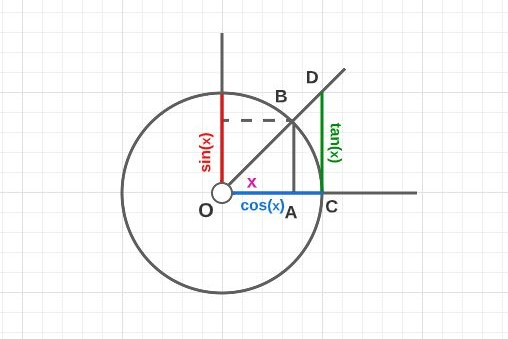
\includegraphics[width=9cm]{images/lim_notevole1.JPG}
            \caption{Dimostrazione limite del seno}
            \label{fig:lim_notevole1}
        \end{figure}
        
        Dalla Figura \ref{fig:lim_notevole1} ricavo i seguenti dati: $\overline{OB}=1$, $\overline{OA}=\cos x$, $\overline{AB}=\sin x$, $\overset{\frown}{BC}=x$, $0<x<\frac{\pi}{2}$.
        
        $O\widetriangle{A}B\simeq O\widetriangle{C}D\Rightarrow\frac{\overline{BA}}{\overline{OA}}=\frac{\overline{DC}}{\overline{OC}}\Rightarrow\frac{\sin x}{\cos x}=\frac{\overline{DC}}{1}=\tan x$.
        
        Quindi posso affermare che:
        \begin{equation}\label{eq:lim_notevole1}
            \overline{AC}\leq \overset{\frown}{BC}\leq\overline{DC} \text{ ovvero } \sin x\leq x\leq\tan x    
        \end{equation}
        
        
        Soffermandoci sulla prima parte possiamo dire che $\overline{AC}\leq \overset{\frown}{BC}$ perchè:
        \begin{enumerate}
            \item $\overline{AB}\leq\overline{BC}$ per il torema di Pitagora
            \item $\overline{BC}\leq\overset{\frown}{BC}$ perchè essendo il segmento la linea più breve per unire due punti, è sicuramente minore dell'arco di circonferenza.
        \end{enumerate}
        
        Per quando riguarda la seconda parte, invece, possiamo dire che $O\widetriangle{C}B\leq O\widetriangle{C}D$, perchè il primo è incluso nel secondo.
        
        Dato che l'area di $O\widetriangle{C}B=\frac{x}{2}$ e l'area di $O\widetriangle{C}D=\frac{\tan x}{2}$.
        Abbiamo che:
        \begin{equation*}
            \frac{x}{2}\leq\frac{\tan x}{2}\Rightarrow x\leq\tan x
        \end{equation*}
        
        Ritornando alla formula \ref{eq:lim_notevole1} abbiamo ottenuto che $\sin x\leq x\leq\tan x$. Volendo ricondurre l'uguaglianza nella forma $\frac{\sin x}{x}$ posso dividere per $\sin x$ e ne derivo:
        \begin{equation*}
            1\leq\frac{x}{\sin x}\leq\frac{1}{\cos x}
        \end{equation*}
        Non mi resta che elevare alla -1 e invertire il verso della disequazione:
        \begin{equation*}
            \cos x\leq\sin x\leq 1    
        \end{equation*}
        
        Considero infine $\cos x=f(x), \frac{\sin x}{x}=g(x), 1=h(x)$ e applico il teorema dei carabinieri (vedi Sezione \ref{td_carabinieri}).
        
        \begin{equation*}
            \lim_{x\to 0}\cos x=1\hspace{0,5cm}\lim_{x\to 0}1=1
        \end{equation*}
        Quindi:
        \begin{equation*}
            \lim_{x\to 0}\frac{\sin x}{x}=1
        \end{equation*}
        
    \end{dimostration}
    
    Da questo limite derivano, attraverso piccole manipolazioni algerbriche, tutti gli altri limiti notevoli trigonometrici.
    Uno tra questi è:
    
    \item $\lim_{x\to 0}\frac{1-\cos x}{x^2}=\frac{1}{2}$
    
    Infatti per ricondurlo al limite \ref{lim:sin} posso moltiplicare e dividere per $1\pm\cos x$.
    
    $\lim_{x\to 0}\frac{(1-cos^{2}x)}{x^{2}(1+cosx)}= \lim_{x\to 0}\frac{sin^{2}x}{x^{2}(1+cosx)}$
    
    Ora come sappiamo il limite di $\frac{\sin x}{x}=1$, quindi:
    
    $\lim_{x\to 0} \frac{sinx}{x}\frac{sinx}{x}\frac{1}{1+cosx}=\frac{1}{2}$.
    \begin{example}
        $\lim_{x\to 0}\frac{\tan x}{x}$
        
        $\lim_{x\to 0}\frac{\tan x}{x}=\lim_{x\to 0}\frac{\sin x}{\cos x*x}=\frac{1}{\cos x}=1$
    \end{example}
\end{enumerate}
Un'altro limite notevole fondamentale è:
\begin{enumerate}[label=\textbf{\arabic*})]\setcounter{enumi}{2}
    \item \label{lim:frac1x} $\lim_{x\to\infty} (1+\frac{1}{x})^{x}=e$
    
    $e$ si chiama numero di Nepero, il cui valore è circa 2,718...
    Quindi possiamo scrivere $\lim_{x\to+\infty} (1+\frac{1}{x})^{x}=e\sim 2,72$.
    \begin{dimostration}
    Per dimostrarlo dobbiamo neccessariamente fare uso del binomio di Newton visto nella sezione \ref{sec:binomio_Newton}.
    
    Applicando quanto visto, in una formula sola otteniamo:
    \begin{equation*}
        (a+b)^n=\sum_{k=0}^n\binom{n}{k}a^{n-k}b^k
    \end{equation*}
    Applicando al limite \ref{lim:frac1x} otteniamo:
    \begin{equation}
        a_n=(a+\frac{1}{x})^x=\sum_{k=0}^n\binom{n}{k}1^{n-k}+\binom{1}{n}^k\text{ ... }
    \end{equation}
    Ora posso scrivere $a_n$ come: $a_n=\binom{n}{0}1^n\binom{1}{n}^0+\binom{n}{1}1^{k-1}\binom{1}{n}^n+\sum_{k=2}^n\binom{n}{k}1^{n-k}\binom{1}{n}^k$
    
    Dove con un pò di ragionamento notiamo come i primi due termini tendono a 1 mentre la sommatoria è $\geq$ 0.
    Quindi avremo che $1+1+\sum_{k=2}^n\binom{n}{k}1^{n-k}\binom{1}{n}^k\geq 2$.
    
    Possiamo scrivere $a_n=2+\sum_{k=2}^n\frac{1}{k!}\frac{n}{n}\frac{n-1}{n}\frac{n-2}{n}\text{ ... }\frac{n-k+1}{n}$ dove tutti i termini dopo $\frac{1}{k!}$ sono $\leq 1$.
    Con gli ultimi due passaggi abbiamo invece che $2+\sum_{k=0}^n\frac{1}{k!}\leq 2+\sum_{k=2}^n\frac{1}{2^{k-1}}=$\\
    $=\sum_{k=2}^n\frac{1}{2}+\frac{1}{2^2}+\text{ ... }+\frac{1}{2^{n1}}=\frac{1}{2}+\frac{1}{4}+\frac{1}{8}+\frac{1}{16}+\text{ ... }+\frac{1}{2^{n-1}}$
    
    Per semplificarci il calcolo disegnamo le frazioni come fette di una torta e notiamo come $a_n$ è sempre contenuta tra 2 e 3.
    Quindi abbiamo dimostrato che $2\leq a_n\leq 3$, $\forall n\in\mathbb{N}$
    
    Ricordiamo che sia $a_n$ monotona crescente o decrescente allora il $\lim_{x\to+\infty}a_n$ esiste e vale $sup_{n=\mathbb{N}}\{a_n\}$. Applicando quanto detto ad $a_n=(1+\frac{1}{n})^n$ ne voglio dedurre il limite.
    Il procedimento non è così immediato perchè $n$ fa riferimeto ai numeri naturali mentre la $x$ del limite \ref{lim:frac1x} appartiene ai numeri reali. Vogliamo quindi generalizzare il tutto ad un insieme più grande.
    
    Dato $x\geq 1$, $\exists !n\in\mathbb{N}$ t.c. $x\leq x\leq n+1$, ovvero x è compreso tra due numeri naturali, dico che:
    \begin{equation*}
        (1+\frac{1}{n+1})^n \leq (1+\frac{1}{x})^x \leq (1+\frac{1}{n})^{n+1}
    \end{equation*}
    Con qualche manipolazione algebrica otteniamo:
    \begin{equation*}
        \frac{a_n+1}{1+\frac{1}{n+1}}\leq (1+\frac{1}{x})^x\leq a_n(1+\frac{1}{n})
    \end{equation*}
    Dove $a_n$ tende ad $e$. Per il teorema dei carabinieri anche il $\lim_{x\to+\infty}(1+\frac{1}{x})^x=e$.
    \end{dimostration}
    
    \item \label{lim:ln}$\lim_{x\to 0} \frac{ln(1+x)}{x}=1$
    
    Il nostro obiettivo è ricondurre il limite nella forma del limite \ref{lim:frac1x}.
    Infatti $\frac{\ln(1+x)}{x}=\frac{1}{x}\ln(1+x)$. Possiamo ora riscrivere l'equazione come $\ln(1+x)^{\frac{1}{x}}$, tramite il cambio di variabile poniamo $y=\frac{1}{x}$ quindi $\lim_{y\to+\infty}\ln(1+\frac{1}{y})^{y}$ che per il limite \ref{lim:frac1x} è uguale a $\ln e=1$.
\end{enumerate}
Anche con le altre basi avviene lo stesso procedimento per cui abbiamo che
\begin{enumerate}[label=\textbf{\arabic*})]\setcounter{enumi}{4}
    \item \label{lim:log} $\lim_{x\to 0} \frac{log_{a}(1+x)}{x}=log_{a}e$
    
    Perchè possiamo moltiplicare e dividere per il $\ln_a$ che ci permette di semplificare. Otteniamo così che il $\lim_{x\to 0} \frac{\log_{a}(1+x)}{x}=\lim_{x\to 0}\frac{\ln_a(1+x)}{x}\frac{1}{\ln a}$. Per il limite \ref{lim:ln} otteniamo $\frac{1}{\ln_a}$.
    
    \item $\lim_{x\to 0}\frac{e^{x}-1}{x}=1$
    
    Vogliamo ricondurlo alla forma del limite \ref{lim:ln}. Per farlo poniamo $y=e^{x}-1$.
    
    Stando a quanto detto $x=\ln(y+1)$ allora otteniamo $\lim_{y\to 0}\frac{y}{ln(y+1)}$. Elevando alla $-1$ otteniamo $\lim_{y\to 0}(\frac{ln(y+1)}{y})^{-1}$ che per il limite \ref{lim:ln} vale $1^{-1}=1$.
\end{enumerate}


\section{Teoremi dei limiti}
\subsection{Teorema dell'unicità del limite}
    A volte i limiti pottono non esistere in tutto $\mathbb{R}$, come il $\lim_{x\to\pm\infty}\sin x$.
    Il problema nasce perchè il $\sin x$ oscilla tra $\pm 1$ e per tanto non si avvicinerà mai a $\pm\infty$.
    
    Stando a quanto detto, se il $\lim_{x\rightarrow x_0/\pm\infty}f(x)$ \textbf{esiste allora è unico}.

    \begin{dimostration}
        Supponiamo, per assurdo, che esistano due valori, $l$, $m\in\mathbb{R}$ con $m<l$ t.c. $\lim_{x \to x_0}f(x)=l$ e $\lim_{x \to x_0}f(x)=m$.
        
        Per definizione di limite risulta che, comunque si fissi $\epsilon>0$, si riescono a determinare due numeri reali $\delta_m>0$ e $\delta_l>0$ tali che, se $0<|x-x_0|<\delta_m$ e $0<|x-x_0|<\delta_l$. Allora $|f(x)-m|<\epsilon$ e $|f(x)-l|<\epsilon$. 
        
        Poniamo $0<\epsilon<\frac{l-m}{2}$  e consideriamo un nuovo $\delta=\min(\delta_l,\delta_m)$, in modo che $x$ soddisfa la relazione
        $0<|x-x_0|<\delta$, e quindi soddisfa anche le due condizioni sopra. 
        
        Svolgendo il sistema di due disuguaglianze grazie alla condizione $m<l$, si ha che $\epsilon>\frac{l-m}{2}$, il che va in contraddizione con la definizione data a $\epsilon$, ottenendo un assurdo. Dunque il limite necessariamente deve essere unico.\flushright{$\blacksquare$}

    \end{dimostration}


\subsection{Teorema del cambio di variabile}
Siano $f:A\subset\mathbb{R}\rightarrow\mathbb{R}$ e $g:B\subset\mathbb{R}\rightarrow\mathbb{R}$.
Supponiamo che:
\begin{enumerate}[label=(\alph*)]
    \item $\lim:{y\to y_0}g(y)=l$;
    \item $\lim_{x\to x_0}f(x)=y_0$;
    \item $f(x)\neq y_0$.
\end{enumerate}
Allora:
\begin{equation}
    \lim_{x\to x_0}g(f(x))=l
\end{equation}

\begin{example}
    $\lim_{x\to 0^+}e^{\frac{1}{x}}$
    
    Mi chiedo la funzione più interna ($\frac{1}{x}$) a quali valori tende a $0^+$? A $+\infty$.
    Quindi $\overline{y=\frac{1}{x}}$ e il risultato sarà quindi $\lim_{y\to +\infty}e^y=+\infty$
\end{example}
\begin{example}
    $\lim_{x\to +\infty}\cos(\frac{x+2}{x^3-1})$\\
    $\overline{y=\frac{x+2}{x^3-1}}$\\
    $\lim_{y\to 0}\cos y=1$
\end{example}
\begin{example}
    $\lim_{x\to +\infty}\frac{\ln^2x-\ln x}{3\ln x+2}$\\
    $\overline{y=\ln x}$\\
    $\lim_{x\to +\infty}\frac{y^2-y}{y+2}=+\infty$
\end{example}


\subsection{Teorema dei due carabinieri}\label{td_carabinieri}
Siano $f,g,h:A\subset\mathbb{R}\rightarrow\mathbb{R}$ supponiamo che $\lim_{x\to x_0}f(x)=\lim_{x\to x_0}h(x)=l$.

\begin{figure}[ht]
    \centering
    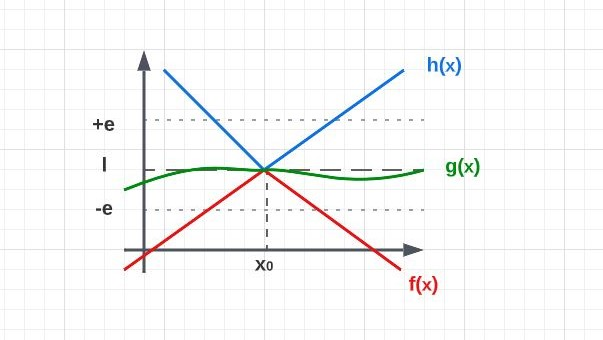
\includegraphics[width=10cm]{images/f_carabinieri.JPG}
    \caption{Funzione dei carabinieri}
    \label{fig:f_carabinieri}
\end{figure}

Sia anche $f(x)\leq g(x)\leq h(x)$ per $x$ vicino a $x_0$. Allora:
\begin{equation}
    \lim_{x\to x_0}g(x)=l
\end{equation}
\begin{osservation}[Fun fact]
    Si chiama teorema dei carabinieri perchè possiamo immaginare le funzioni $f$ ed $h$ come dei carabinieri che per $x_0$ tentano di catturare il ladro (funzione $g$). Tutte e tre le funzioni tendono a $l$.
\end{osservation}
\begin{dimostration}
Dimostriamo quanto detto:
    \begin{enumerate}
    
        \item $\lim_{x\to x_0}f(x)=l$
        
        $\forall\epsilon>0,\exists\delta_1>0\text{ t.c. }l-\epsilon<f(x)<l+\epsilon, \forall x\in A\text{ con } 0<|x-x_0|<\delta_1$
        \item $\lim_{x\to x_0}h(x)=l$;
        
        $\forall\epsilon>0,\exists\delta_2>0\text{ t.c. }l-\epsilon<h(x)<l+\epsilon, \forall x\in A\text{ con } 0<|x-x_0|<\delta_2$.
    \end{enumerate}
    Inoltre $\exists\delta_0>0\text{ t.c. }f(x)<g(x)<h(x), \forall x\in A\text{ con }0<|x-x_0|<\delta_0$.
    
    A questo punto scelgo $\delta$ come il minimo tra $\delta_0,\delta_1,\delta_2$.
    Quindi per $x\in A\text{ t.c. } 0<|x-x_0|<\delta$ valgono:
    \begin{enumerate}
        \item $l-\epsilon<f(x)<l+\epsilon$;
        \item $l-\epsilon<h(x)<l+\epsilon$;
        \item $f(x)<g(x)<h(x)$.
    \end{enumerate}
    
    Quindi $l-\epsilon<f(x)<g(x)<h(x)<l+\epsilon$ abbiamo dimostrato che vale anche per $l-\epsilon<g(x)<l+\epsilon$. Ovvero:
    \begin{equation}
        \lim_{x\to x_0}g(x)=l
    \end{equation}
\end{dimostration}


\subsection{Teorema della permanenza del segno}
Consideriamo la funzione $f(x)$ e un punto $c\in dom(f)$. Se il limite di $x\to c$ di $f(x)$ è ugule a $l\in\mathbb{R}$, allora esiste un intorno di c in cui la funzione assume lo stesso segno del limite.

In particolare:
\begin{itemize}
    \item se $\lim_{x\to c}f(x)=l>0$ allora $f(x)>0$;
    \item se $\lim_{x\to c}f(x)=l<0$ allora $f(x)<0$.
\end{itemize}

\begin{dimostration}
    Per ipotesi sapiamo che il $\lim_{x\to c}f(x)=l$ esiste ed è finito.
    
    Quindi da $\forall\epsilon>0,\exists\delta>0\text{ t.c. }|f(x)-l|<\epsilon, \forall x\in A\text{ con } 0<|x-c|<\delta$ otteniamo $l-\epsilon<f(x)<l+\epsilon$.
    
    Notiamo come questa relazione valga per ogni $\epsilon$, abbiamo pertanto la possibiltà di sceglierne il valore a patto che sia maggiore di 0. Possiamo quindi scrivere $\epsilon=\frac{|l|}{2}$.
    
    La relazione diventerà $l-\frac{|l|}{2}<f(x)<l+\frac{|l|}{2}$. E considerando $l$ positivo otteniamo $\frac{l}{2}<f(x)<\frac{3}{2}l$ mentre considerando $l$ negativo otteniamo $\frac{3}{2}l<f(x)<\frac{l}{2}$.
    
    In entrabi i casi la funzione segue il segno di $l$.\flushright{$\blacksquare$}
\end{dimostration}

\subsection*{Teorema dei gradi}\label{subsec:tdg}
Il teorema dei gradi ci permette di risolvere i $\lim_{x\to\pm\infty f(x)}$ dove $f(x)$ è una funzione fratta del tipo $\frac{P(x)}{Q(x)}$. Ci possono essere tre casi:
\begin{enumerate}
    \item Se gradi delle x del numeratore e denominatore sono uguali $GN=GD$, il risultato sarà il rapporto tra i coefficienti $\frac{a}{b}$;
    \item Se il grado del numeratore è maggiore del grado del denominatore $GN>GD$, il risultato sarà $\pm\infty$ a seconda dei calcoli;
    \item Se grado del denominatore è maggiore del grado del numeratore $GN<GD$, il risultato sarà 0.

\end{enumerate}

\subsection*{Teorema del confronto}
Siano $f,g:f(x)\leq g(x)$ per $x$ vicino a $x_0$. Supponiamo che $\lim_{x\to x_0}f(x)=+\infty$ allora $\lim_{x\to x_0}g(x)=+\infty$
\begin{example}
    \begin{equation*}
        \lim_{x\to +\infty}(2+\cos x)^x \text{ non esiste}
    \end{equation*}
    Mentre:
    \begin{equation*}
        \lim_{x\to +\infty}(3+\cos x)^x=+\infty    
    \end{equation*}
    Perchè nel primo caso la funzione cresce per un certo valore e poi torna ad 1 (per l'andamento del $\cos$), perchè il $\cos$ oscilla tra $[3;1]$. Nel secondo caso invece il $\cos$ apparentemente oscilla tra $[4;2]$ ma in realtà non torna a 2 ma cresce all'infinito.
    
    Volendo applicare il teorema sopra descritto abbiamo che $f(x)=2^x$, $g(x)=(3+\cos x)^x$. Quindi otteniamo che:
    \begin{equation*}
        \lim_{x\to +\infty}f(x)=\lim_{x\to +\infty}2^x=+\infty
    \end{equation*}
    \begin{equation*}
        \lim_{x\to +\infty}g(x)=\lim_{x\to +\infty}(3+\cos x)^x=+\infty
    \end{equation*}
\end{example}

\begin{dimostration}
    Per assurdo ipotizziamo $l_1>l_2$. Siano $V_1$, intorno di $l_1$ e $V_2$ intorno di $l_2$ t.c. $V_1\land V_2\neq\emptyset$. In particolare $y_1>y_2$, $\forall y_1\in V_1$ e $\forall y_2\in V_2$.
    
    Dalla definizione di limite, per $V_1$, $\exists U_1$, introno di $x_0$ t.c. $f(x)\in V_1$, $\forall x \in A\land(U_1\backslash\{x_0\})$.
    
    Dalla definizione di limite, per $V_2$, $\exists U_2$, introno di $x_0$ t.c. $f(x)\in V_2$, $\forall x \in A\land(U_2\backslash\{x_0\})$.
    
    Inoltre $f(x)\leq g(x)$ definitivamente per $x\to0$. $\exists U_0$ intorno di $x_0$ t.c. $f(x)\leq g(x)$ per $x\in A\land(U_0\backslash\{x_0\})$.
    
    Sia $U=U_0\land U_1\land U_2$. Per $x\in A\land(U\backslash\{x_0\})$ valgono:
    \begin{enumerate}
        \item $f(x)\in V_1$
        \item $g(x)\in V_2$
        \item $f(x)\leq g(x)$
    \end{enumerate}
\end{dimostration}

\section{Successioni}
\begin{definition}[Successione]
    Una successione è una funzione il cui dominio è in $\mathbb{N}$. Se il codominio è contenuto in $\mathbb{R}$ la successione si chiama reale.
\end{definition}
\begin{example}
    Se scrivo $a_n=\sqrt{n^2+1}$ intendo la funzione $f\mathbb{N}\rightarrow\mathbb{R}$ data da $a_n=\sqrt{n^2+1}$. Quindi se $n=$
    \begin{table}[ht]
        \centering
        \begin{tabular}{ccl}
            0 & $\rightarrow$ & $\sqrt{0^2+1}=1$ \\
            1 & $\rightarrow$ & $\sqrt{2}$\\
            2 & $\rightarrow$ & $\sqrt{5}$\\
            3 & $\rightarrow$ & $\sqrt{10}$\\
        \end{tabular}
    \end{table}
\end{example}

Graficamente posso rappresentare una funzione reale in due modi: come grafico della funzione o come punti su una retta reale.

\begin{figure}[htp]
    \centering
    
    \begin{minipage}[b]{.3\columnwidth}
        \centering
        \hfill
         \begin{tikzpicture}
            % Assi
            \draw[->,thick] (0,0) -- (4.5,0);
            \draw[->,thick] (0,-2.5) -- (0,2.5);
            % Numeri
            \draw (1,0) -- (1,0.1) node [above] {\small{1}};
            \draw (2,0) -- (2,0.1) node [above] {\small{2}};
            \draw (3,0) -- (3,0.1) node [above] {\small{3}};
            \draw (4,0) -- (4,0.1) node [above] {\small{4}};
            \draw (0,-0.5) -- (-0.2,-0.5) node [above] {\small{-1}};
            \draw (0,-1.5) -- (-0.2,-1.5) node [above] {\small{-3}};
            \draw (0,1) -- (-0.2,1) node [above] {\small{2}};
            \draw (0,2) -- (-0.2,2) node [above] {\small{4}};
            % Punti
            \filldraw[black] (1,-0.5) circle (1.5pt);
            \filldraw[black] (3,-1.5) circle (1.5pt);
            \filldraw[black] (2,1) circle (1.5pt);
            \filldraw[black] (4,2) circle (1.5pt);
        \end{tikzpicture}
        
        \caption{Successione con grafico della funzione}
    \end{minipage}\hfill
    \begin{minipage}[b]{.3\columnwidth}
        \centering
        
        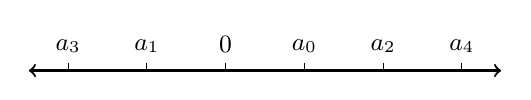
\begin{tikzpicture}
            % Assi
            \draw[<->,thick] (-2.5,0) -- (3.5,0);
            % Numeri
            \draw (0,0) -- (0,0.1) node [above] {\small{0}};
            \draw (1,0) -- (1,0.1) node [above] {\small{$a_0$}};
            \draw (2,0) -- (2,0.1) node [above] {\small{$a_2$}};
            \draw (3,0) -- (3,0.1) node [above] {\small{$a_4$}};
            \draw (-1,0) -- (-1,0.1) node [above] {\small{$a_1$}};
            \draw (-2,0) -- (-2,0.1) node [above] {\small{$a_3$}};
        \end{tikzpicture}
        
        \caption{Successione con punti sulla retta}
    \end{minipage}\hspace*{\fill}
\end{figure}

\textbf{Altre notazioni per indicare una successione:}
\begin{equation*}
    \{a_n\} n\in\mathbb{N} \hspace{0,5cm} (a_n) n\in\mathbb{N} \hspace{0,5cm} \{a_n\} n\geq 1 \hspace{0,5cm} \{a_n\} n\geq n_0
\end{equation*}

Più interessante è sicuramente vedere il $\lim_{n\to\infty}$ di una successione.

Analogamente al $\lim_{x\to+\infty}f(x)$ possiamo definire:
\begin{equation}\label{eq:lim_succe}
    \lim_{n\to+\infty}a_n=l
\end{equation}

Se $l\in\mathbb{R}$, \ref{eq:lim_succe} vuol dire che $\forall\epsilon>0, \exists N\in\mathbb{N}$ t.c. $|a_n-l|<\epsilon, \forall n>N$.

Se $l=+\infty$, \ref{eq:lim_succe} vuol dire che $\forall M\in\mathbb{N}, \exists N\in\mathbb{N}$ t.c. $a_n>M(<M), \forall n>N$.

\begin{center}
    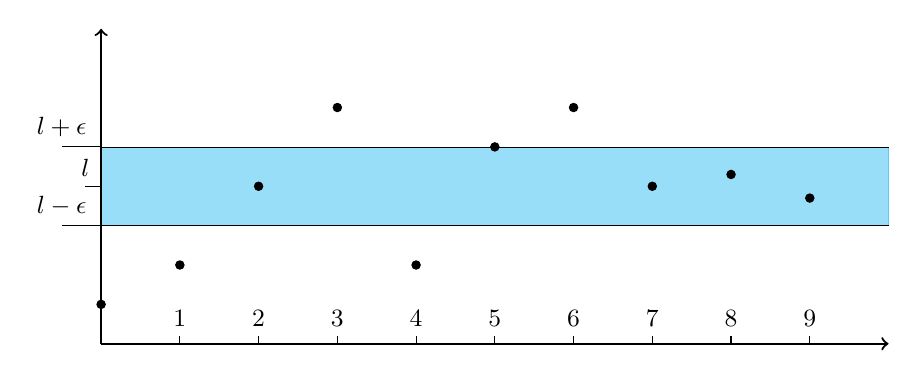
\begin{tikzpicture}
        % Assi
        \draw [fill=cyan,cyan, very thin, opacity=0.4] (0,1.5) rectangle (10,2.5); 
        \draw [->,thick] (0,0) -- (10,0);
        \draw [->,thick] (0,0) -- (0,4);
        \draw [very thin] (0,1.5) -- (10,1.5);
        \draw [very thin] (0,2.5) -- (10,2.5);
        % Numeri
        \draw (1,0) -- (1,0.1) node [above] {\small{1}};
        \draw (2,0) -- (2,0.1) node [above] {\small{2}};
        \draw (3,0) -- (3,0.1) node [above] {\small{3}};
        \draw (4,0) -- (4,0.1) node [above] {\small{4}};
        \draw (5,0) -- (5,0.1) node [above] {\small{5}};
        \draw (6,0) -- (6,0.1) node [above] {\small{6}};
        \draw (7,0) -- (7,0.1) node [above] {\small{7}};
        \draw (8,0) -- (8,0.1) node [above] {\small{8}};
        \draw (9,0) -- (9,0.1) node [above] {\small{9}};
        \draw (0,2) -- (-0.2,2) node [above] {\small{$l$}};
        \draw (0,1.5) -- (-0.5,1.5) node [above] {\small{$l-\epsilon$}};
        \draw (0,2.5) -- (-0.5,2.5) node [above] {\small{$l+\epsilon$}};
        % Punti
        \filldraw[black] (0,0.5) circle (1.5pt);
        \filldraw[black] (1,1) circle (1.5pt);
        \filldraw[black] (2,2) circle (1.5pt);
        \filldraw[black] (3,3) circle (1.5pt);
        \filldraw[black] (4,1) circle (1.5pt);
        \filldraw[black] (5,2.5) circle (1.5pt);
        \filldraw[black] (6,3) circle (1.5pt);
        \filldraw[black] (7,2) circle (1.5pt);
        \filldraw[black] (8,2.15) circle (1.5pt);
        \filldraw[black] (9,1.85) circle (1.5pt);
    \end{tikzpicture}
\end{center}

Se quindi avendo la restrizione della funzione sei numeri reali, ne so derivare il limite, allora posso calcolare anche il limite della sua successione.

\textbf{\large{Successioni interessanti:}}%\normalsize{}

\begin{itemize}
    \item[] $\{n^\alpha\}_{n\geq1}$ $\alpha\in\mathbb{R}$
    \item[] $\{a^n\}_{n\geq1}$ $a\in\mathbb{R}$
    \item[] $\{log_an\}_{n\geq1}$ $a>0$ $a\neq 1$
    \item[] $\{n!\}$ $n\geq0$
\end{itemize}
Quindi:
\begin{itemize}
    \item[] $\lim_{n\to+\infty}n!=+\infty$
    \item[] $\lim_{n\to+\infty}n^\alpha=\begin{cases}
                0 \text{ se } \alpha<0\\
                1 \text{ se } \alpha=0\\
                +\infty \text{ se } \alpha>0\\
            \end{cases}$
    \item[] $\lim_{n\to+\infty}a^n=\begin{cases}
                +\infty \text{ se } a>1\\
                0 \text{ se } -1<a<1\\
                \text{non esiste se } a\leq-1\\
            \end{cases}$
    \item[] $\lim_{n\to+\infty}\log_an=\begin{cases}
                +\infty \text{ se } a>1\\
                -\infty \text{ se } 0<a<1\\
            \end{cases}$
\end{itemize}

\textbf{\large{Gerarchia degli infiniti}}

Ci sono inoltre delle funzioni che vanno più velocemente di altre a $\pm\infty$.
Quindi dire che $a_n\ll b_n$ vuol dire che $\lim_{x\to+\infty}\frac{a_n}{b_n}=0$ oppure $\lim_{x\to+\infty}\frac{b_n}{a_n}=+\infty$.
Gerarchie da ricordare:
\begin{equation*}
    \log_an\ll n^\alpha\ll a^n\ll n!\ll n^n
\end{equation*}

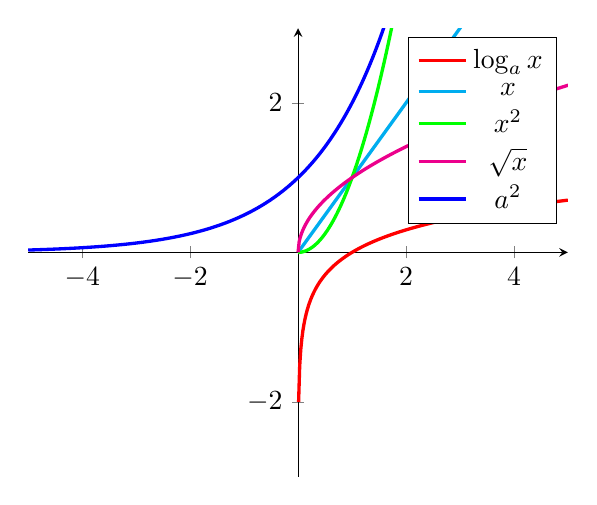
\begin{tikzpicture}
    \begin{axis}[xmin=-5,xmax=5,ymin=-3,ymax=3,axis x line=middle, axis y line=middle]
    \addplot [very thick,domain=-5:5,samples=500,color=red,]{log10(x)};\addlegendentry{$\log_ax$}
    \addplot [very thick,domain=0:10,samples=500,color=cyan,]{x};\addlegendentry{$x$}
    \addplot [very thick,domain=0:10,samples=500,color=green,]{x^2};\addlegendentry{$x^2$}
    \addplot [very thick,domain=0:10,samples=500,color=magenta,]{sqrt(\x)};\addlegendentry{$\sqrt{x}$}
    \addplot [very thick,domain=-5:5,samples=500,color=blue,]{2^x};\addlegendentry{$a^2$}
    \end{axis}
\end{tikzpicture}

Per le funzioni di x vale qualcosa di analogo. In generale $f(x)\ll g(x)$ se $\lim_{x\to+\infty}\frac{f(x)}{g(x)}=0$.

Da questa gerarchia degli infiniti ne otteniamo una analoga per $x\to0$ con dei cambi di variabile.

\textbf{\large{Successione limitata}}
\begin{definition}[Successione limitata]
    Una successione si dice limitata se $\exists M\geq 0\text{ t.c. }|a_n|\leq M, \forall n\in\mathbb{N}$.
\end{definition}


\subsection{Sottosuccessioni}
\begin{definition}[Sottosuccessione]
    Data una successione $\{a_n\}_{n\in\mathbb{N}}$ una sottosuccessione è una nuova successione $\{\widetilde{a_n}\}_{n\in\mathbb{N}}$, così defnita: presa una funzione crescente $\mathbb{R}:\mathbb{N}\rightarrow\mathbb{N}$ e si definisce $\widetilde{a_n}:=a_{f(n)}$.
\end{definition}

Una sottosuccessione è quindi una successione senza alcuni valori.

\begin{center}
    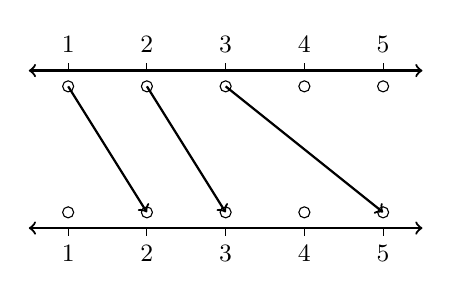
\begin{tikzpicture}
        \draw[<->,thick] (0,0) -- (5,0);
        \draw (0.5,0) -- (0.5,0.1) node [above] {\small{1}};
        \draw (1.5,0) -- (1.5,0.1) node [above] {\small{2}};
        \draw (2.5,0) -- (2.5,0.1) node [above] {\small{3}};
        \draw (3.5,0) -- (3.5,0.1) node [above] {\small{4}};
        \draw (4.5,0) -- (4.5,0.1) node [above] {\small{5}};
        \draw[black] (0.5,-0.2) circle (2pt);
        \draw[black] (1.5,-0.2) circle (2pt);
        \draw[black] (2.5,-0.2) circle (2pt);
        \draw[black] (3.5,-0.2) circle (2pt);
        \draw[black] (4.5,-0.2) circle (2pt);
        
        \draw[<->,thick] (0,-2) -- (5,-2);
        \draw (0.5,-2) -- (0.5,-2.1) node [below] {\small{1}};
        \draw (1.5,-2) -- (1.5,-2.1) node [below] {\small{2}};
        \draw (2.5,-2) -- (2.5,-2.1) node [below] {\small{3}};
        \draw (3.5,-2) -- (3.5,-2.1) node [below] {\small{4}};
        \draw (4.5,-2) -- (4.5,-2.1) node [below] {\small{5}};
        \draw[black] (0.5,-1.8) circle (2pt);
        \draw[black] (1.5,-1.8) circle (2pt);
        \draw[black] (2.5,-1.8) circle (2pt);
        \draw[black] (3.5,-1.8) circle (2pt);
        \draw[black] (4.5,-1.8) circle (2pt);
        
        \draw[->,thick] (0.5,-0.2) -- (1.5,-1.8);
        \draw[->,thick] (1.5,-0.2) -- (2.5,-1.8);
        \draw[->,thick] (2.5,-0.2) -- (4.5,-1.8);
    \end{tikzpicture}
\end{center}

Ad esempio la successione $a_n=\frac{1}{n}=1,\frac{1}{2},\frac{1}{3},\frac{1}{4},...$ può generare la sottosuccessione $\widetilde{a_n}=a_{2n}=\frac{1}{2},\frac{1}{4},\frac{1}{6},...$

Immaginiamo ora una successione che sta convergendo ad $l$. Trovare una sottosuccessione significa prendere alcuni dei punti della successione, pertanto anche la sottosuccessione tende a $l$. Ma dobbiamo stare attenti perchè questo ragionamento non vale viceversa.

\begin{example}
    $a_n=(-1)^n$ non ha limite.
    
    La sottosuccessione dei numeri pari $\widetilde{a_n}=a_{2n}=1$, invece, ammette il limite $\lim_{x\to+\infty}\widetilde{a_n}=1$.
\end{example}

Dato l'esempio precedente possiamo quindi chiederci, data una qualunque successione, è possible trovare una sottosuccesione convergente (il limite è finito)?

La risposta è affermativa ma per dimostrarlo, dobbiamo introdurre un nuovo teorema.

\subsection{Teorema di Bolzano-Weierstrass}
Il teorema di Bolzano-Weierstrass afferma che ogni successione $\{a_n\}$ limitata contiene una sottosuccessione convergente.

Ricordiamo che ogni successione monotona crescente (decrescente), ammette un limite che vale $\lim_{x\to+\infty}x_n=sup(inf)\{x_n, n\in\mathbb{N}\}$.

\begin{dimostration}
    Sia $x_0=-M, y_0=M, I_0=[x_0,y_0]=[-M,M]$, scelgo $\widetilde{a_0}=a_0\in I_0$.
    
    \begin{center}
    \begin{tikzpicture}
        % Assi
        \draw [<->,thick] (0,0) -- (10,0);
        % Numeri
        \draw (1,0) -- (1,0) node [below] {\small{$x_0$}};
        \draw (2,0) -- (2,0) node [below] {\small{$a_3$}};
        \draw (3,0) -- (3,0) node [below] {\small{$a_0$}};
        \draw (4,0) -- (4,0) node [below] {\small{$a_1$}};
        \draw (5,0) -- (5,0) node [below] {\small{0}};
        \draw (6,0) -- (6,0) node [below] {\small{$a_4$}};
        \draw (7,0) -- (7,0) node [below] {\small{$a_2$}};
        \draw (8,0) -- (8,0) node [below] {\small{$a_5$}};
        \draw (9,0) -- (9,0) node [below] {\small{$y_0$}};
        \draw (3,-1) -- (3,-1) node [below] {\small{$I_0$}};
        \draw (4,1) -- (4,1) node [above] {\small{$I_1$}};
        \draw (1,-0.5) -- (1,-0.5) node [below] {\small{$x_1$}};
        \draw (5,-0.5) -- (5,-0.5) node [below] {\small{$y_1$}};
        \draw (5,0.5) -- (5,0.5) node [above] {\small{$y_2$}};
        \draw (3,0.5) -- (3,0.5) node [above] {\small{$x_2$}};
        % other
        \draw (1, -0.5) .. controls (3,-1) .. (5, -0.5);
        \draw (3,0.5) .. controls (4,1) .. (5, 0.5);
    \end{tikzpicture}
\end{center}

Ora dividiamo l'intervallo $I_0$ in due intervalli $[x_0, 0]\text{ e }[0,y_0]$ e scelgo quello in cui cadono infiniti punti della successione. Chiamo questo nuovo intervallo $I_1=[x_1,y_2]$.

A questo punto scelgo $h_1\in\mathbb{N}\text{ t.c. }h(1)>0\text{ e }a_{n_{h_1}}\in I_1$.

Essenzialmente sto prendendo un valore $\widetilde{a_1}=a_{h_1}$.
Posso dividere, ancora una volta, l'intervallo $I_1$ in due parti uguali e scegliere l'intervallo che contenga infiniti elementi. Lo chiamo $I_2=[x_2,y_2]$. Scelgo $h_2\text{ t.c. }\widetilde{a_2}=a_{h_2}\in I_2\text{ e }h_2>h_1$, in modo tale che la successione cresca sempre di valori.

Procedeno induttivamente posso dire che se ho costruito $I_0>I_1>I_2>\text{...}>I_n$ e $\widetilde{a_0},\text{...},\widetilde{a_n}\text{ t.c. }\widetilde{a_j}=a_{h_j}\in I_j$ e $h_0<h_1<\text{...}<h_n$, costruisco anche $I_{n+1}$, dividendo $I_n$ in due intervalli uguali e scegliendo quello in cui sono contenuti infiniti punti della successione.

Quindi ottengo una successione di intervalli $I_j$ che hanno estremi $[x_j,y_j]\text{ t.c. }I_{j+1}<I_j$. La lunghezza $I_j=y_j-x_j=\frac{M}{2j-1}\rightarrow 0$ perchè le lunghezze diventano sempre più piccole (o il denominatore assume valori sempre maggiori).

Ottengo così una sottosuccessione $\widetilde{a_j}=a_{j_h}\text{ con }\widetilde{a_j}\in I_j$.
\begin{equation*}
    I_{j+1}\subset I_j \iff \begin{cases}
    x_{j+1} \geq x_j\\
    y_{j+1} \leq y_j
    \end{cases}
\end{equation*}
L'intervallo si stringe e la successione è limitata dall'alto.

Quindi $\{x_j\}$ è una successione crescente e ha limite $l\leq M$ (perchè $x_j\leq M$). Allo stesso modo $\{y_0\}$ è decrescente e quindi ha limite $l'\geq -M$. Inoltre poichè $y_j-x_j=\frac{M}{2_j-1}\rightarrow 0$ per $j\to+\infty$, abbiamo che:
\begin{equation*}
    \lim_{x\to+\infty}y_j-x_j=\lim_{x\to+\infty}y_j-\lim_{x\to+\infty}x_j=l'-l
\end{equation*}
\begin{equation*}
    \widetilde{a_j}\in I_j \iff x_j\leq \widetilde{a_j}\leq y_j
\end{equation*}
Dato che $x_j$ e $j_0$ tendono a 0, per il teorema dei due carabinieri:
\begin{equation*}
    \lim_{x\to+\infty}\widetilde{a_j}=l
\end{equation*}
Questo limite esiste ed è finito quindi abbiamo dimostrato che $\{\widetilde{a_j}\}$ è una successione convergente.\flushright{$\blacksquare$}
\end{dimostration}



\section{Funzioni continue}
\begin{definition}[Funzioni continue]
    $f A\subset\mathbb{R}\rightarrow\mathbb{R}$ si dice continua in $x_0\in A$ se:
    \begin{itemize}
        \item $\lim_{x\to x_0}f(x)=f(x_0)$.
        \item $x_0$ è un punto isolato di $A$, ovvero $\exists \delta>0 \text{ t.c. }A\cap(x_o-\delta, x_0+\delta)=\{x_0\}$.
    \end{itemize}
\end{definition}

Se $f$ non è continua in $x_0\in A$, allora si dice discontinua in $x_0$.
Ad esempio: $f(x)=\frac{1}{x}$ è continua in $x_0\forall x_0\in A$, $\forall x_0\in\text{ dom}f=\mathbb{R}\backslash\{0\}$, quindi è continua.

I punti $x_0\in A$ in cui una funzione $f$ non è continua, si dicono punti di discontinuità.
Ad esempio: $F_{[0,+\infty]}$ $(x)=\begin{cases}
    1\text{ se } x\geq 0\\
    0\text{ se } x<0\\
\end{cases}$
Quindi $F_{[0,+\infty]}$ è continua in $x_0,\forall x_0\neq 0$, ma è discontinua in 0.
Infatti il $\lim_{x\to 0}F_{[0,+\infty]}(x)$ non esiste, e se non esiste potrebbe essere uguale a 0.

Ricordiamo la definizione di limite: $\lim_{x\to x_0}f(x)=l\in\mathbb{R}\text{ se } \forall\varepsilon>0,\exists\delta>0:|f(x)-l|<\varepsilon,\forall x\in\text{dom}\cap (x_0-\delta, x_0+\delta)\backslash\{x_0\}$.
Posso così riscrivere la definizione di di continuità usando la definizione di limite. $f$ è continua in $x_0$ se: 
\begin{equation*}
    \forall\varepsilon>0,\exists\delta>0\text{ t.c. }|f(x)-f(x_0)|<\varepsilon,\forall x\in\text{dom}f\text{ con }|x-x_0|<\delta.    
\end{equation*}
Ovvero se nel punto $x_0$ la funzione è esattamente uguale a $f(x_0)$.

\begin{center}
    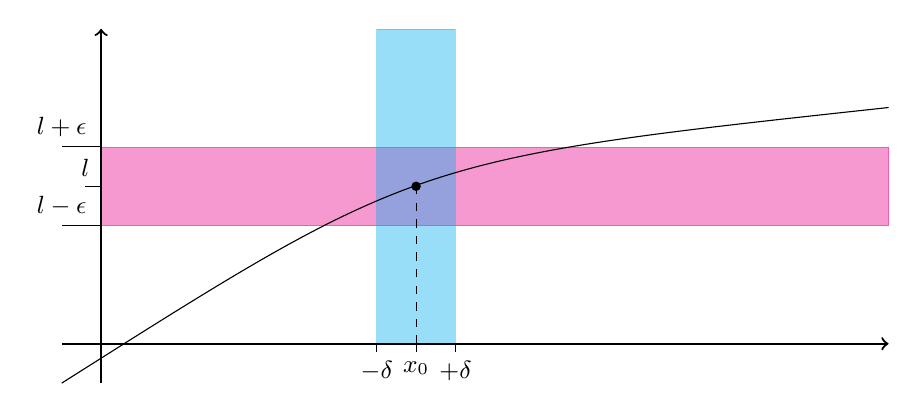
\begin{tikzpicture}
        % Assi
        \draw [fill=magenta,magenta, very thin, opacity=0.4] (0,1.5) rectangle (10,2.5);
        \draw [fill=cyan,cyan, very thin, opacity=0.4] (3.5,0) rectangle (4.5,4); 
        \draw [->,thick] (-0.5,0) -- (10,0);
        \draw [->,thick] (0,-0.5) -- (0,4);
        \draw [dashed] (4,0) -- (4,2);
        \draw (-0.5, -0.5) .. controls (4,2.35) .. (10, 3);
        % Numeri
        \draw (3.5,0) -- (3.5,-0.1) node [below] {\small{$-\delta$}};
        \draw (4,0) -- (4,-0.1) node [below] {\small{$x_0$}};
        \draw (4.5,0) -- (4.5,-0.1) node [below] {\small{$+\delta$}};
        \draw (0,2) -- (-0.2,2) node [above] {\small{$l$}};
        \draw (0,1.5) -- (-0.5,1.5) node [above] {\small{$l-\epsilon$}};
        \draw (0,2.5) -- (-0.5,2.5) node [above] {\small{$l+\epsilon$}};
        % Punti
        \filldraw[black] (4,2) circle (1.5pt);
    \end{tikzpicture}
\end{center}

\begin{osservation}
    Quasi tutte le funzioni che usiamo sono continue (es. funzioni trigonometriche).
\end{osservation}

Con le conoscenze appena apprese possiamo affermare che se $f$ e $g$ sono continue in $x_0$ allora anche $f+g$ è continua in $x_0$.
\begin{dimostration}
    $\lim_{x\to x_0}(f(x)+g(x))$
    
    Per il teorema del limite della somma, questo limite è uguale alla somma dei limiti: $\lim_{x\to x_0}f(x)+\lim_{x\to x_0}g(x)$, per continuità di $f$ e $g$, $f(x_0)+g(x_0)$ è continua.
\end{dimostration}

Allo stesso modo il prodotto, il quoziente e la composizione di funzioni continue, sono sempre funzioni continue.

\subsection*{Continuità di successioni}
Sia $f A\rightarrow\mathbb{R}, x_0\in A$ non isolato. Allora $f$ è continua in $x_0$ se e solo se $\forall\{a_n\}$ successione t.c. $\lim_{x\to x_0}a_n=x_0$, vale:
\begin{equation*}
    \lim_{n\to +\infty}f(a_n)=f(x_0)
\end{equation*}
\begin{dimostration}
    Sia $f$ continua in $x_0$. Sia anche $\{a_n\}_{n\in\mathbb{N}}$ una successione con $\lim_{n\to +\infty}a_n=f(x_0)$. Vogliamo verificare che $\lim_{n\to +\infty}f(a_n)=f(x_0)$, ovvero che $\forall\varepsilon>0, \exists N\in\mathbb{R}\text{ t.c. }|f(x)-f(x_0)|<\varepsilon$ per $x\to x_0, x\in\text{dom}f\cap (x_0-\delta,x_0+\delta)$.
    
    Poichè $\lim_{n\to +\infty}a_n=x_0, \forall\varepsilon'>0, \exists N\in\mathbb{R}\text{ t.c. }|a_n-x_0|<\varepsilon',\forall n>N$.
    Dato che posso scegliere $\varepsilon'>0$ a piacere, scelgo $\varepsilon'=\delta$ come trovato precedentemente. Quindi $\forall n>N, a_n\in\text{dom}f\cap(x_0-\delta,x_0+\delta)$, implica che, $|f(a_n)-f(x)|<\varepsilon$, è ciò che volevamo ottenere.
\end{dimostration}

Proviamo ora a dimostrare l'opposto, ovvero che se per ogni successione $\{a_n\}_{n\in\mathbb{N}}$ t.c. $a_n\to x_0$ per $n\to+\infty$ vale $f(a_n)\rightarrow f(x_0)$ per $n\to+\infty$, allora $f$ è continua in $x_0$, ovvero $\lim_{x\to x_0}f(x)=f(x_0)$.
Lo dimostriamo per assurdo:
\begin{dimostration}
    Ipotizzo che la tesi sia falsa e ottengo una contraddizione.
    
    Quindi ipotizzo che \textbf{non vale} $\lim_{x\to x_0}f(x)=f(x_0)$ ovvero che $\exists\varepsilon>0\text{ t.c. }\forall\delta>0$ non vale $|f(x)-f(x_0)|<\varepsilon, \forall x\in A$ con $|x-x_0|<\delta$, ovvero $\exists a\in A$ con $|a-x_0|<\delta$ t.c. $|f(a)-f(x_0)|\geq\varepsilon$.
    
\begin{center}
    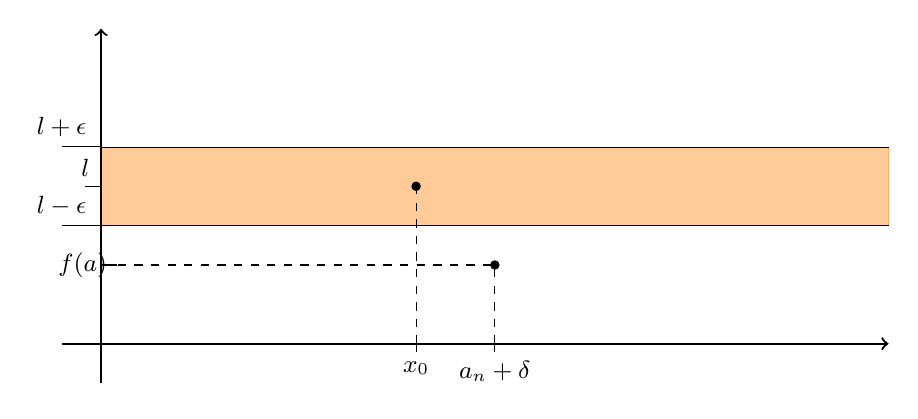
\begin{tikzpicture}
        % Assi
        \draw [fill=orange,orange, very thin, opacity=0.4] (0,1.5) rectangle (10,2.5); 
        \draw [->,thick] (-0.5,0) -- (10,0);
        \draw [->,thick] (0,-0.5) -- (0,4);
        \draw [very thin] (0,1.5) -- (10,1.5);
        \draw [very thin] (0,2.5) -- (10,2.5);
        \draw [dashed] (4,0) -- (4,2);
        \draw [dashed] (5,0) -- (5,1);
        \draw [dashed] (0,1) -- (5,1);
        % Numeri
        \draw (4,0) -- (4,-0.1) node [below] {\small{$x_0$}};
        \draw (5,0) -- (5,-0.1) node [below] {\small{$a_n+\delta$}};
        \draw (0,2) -- (-0.2,2) node [above] {\small{$l$}};
        \draw (0,1.5) -- (-0.5,1.5) node [above] {\small{$l-\epsilon$}};
        \draw (0,2.5) -- (-0.5,2.5) node [above] {\small{$l+\epsilon$}};
        \draw (0,1) -- (0.2,1) node [left] {\small{$f(a)$}};
        % Punti
        \filldraw[black] (4,2) circle (1.5pt);
        \filldraw[black] (5,1) circle (1.5pt);
    \end{tikzpicture}
    
    $f(a)$ non cade nell'intervallo $f(x_0)\pm\delta$.
\end{center}
    
    Ora voglio costruire una successione $\{a_n\}$ con $a_n\to x_0$ ma $f(a_n)\text{ non tende a }f(x_0)$ per $n\to+\infty$. Questo violerà l'ipotesi e creerà una contraddizione.
    
    Per costruire questa successione prendo una successione di $\delta>0$ che vanno a zero (es. $\delta_n=\frac{1}{n}$). Quindi $\exists a_n\in A$ con $|a_n-x_0|<\delta_n$ t.c. $|f(a_n)-f(x_0)|\geq\varepsilon$.
    
    Chiaramente $\lim_{n\to+\infty}a_n=x_0$ ma $\lim_{n\to+\infty}f(a_n)\neq f(x_0)$. Ecco trovato l'assurdo.
\end{dimostration}

\subsection*{Teorema dell'esistenza degli zeri}
Sia $f[a,b]\to\mathbb{R}$ continua, t.c. $f(a)<0$, $f(b)>0$ oppure viceversa. Allora:
\begin{equation*}
    \exists\xi\in (a,b) \text{ t.c. }f(\xi)=0
\end{equation*}
Ovvero che presa una funzione continua in un intervallo $[a,b]$ e dimostrando che cresce passando per 0, allora esisterà sempre il valore $f(0)$ della funzione.

\begin{center}
    \begin{tikzpicture}
        % Assi
        \draw [->,thick] (-0.5,0) -- (10,0);
        \draw [->,thick] (0,-2) -- (0,2);
        \draw (-0.5, -2) .. controls (2,-1.5) .. (4,0);
        \draw (4,0) .. controls (6,1) .. (10,2);
        % Numeri
        \draw (4,0) -- (4,-0.1) node [below] {\small{$\xi$}};
        \draw (1,0) -- (1,-0.1) node [below] {\small{$a$}};
        \draw (8,0) -- (8,-0.1) node [below] {\small{$b$}};
        \draw (0,1.5) -- (-0.5,1.5) node [above] {\small{$f(b)$}};
        \draw (0,-1.5) -- (-0.5,-1.5) node [above] {\small{$f(a)$}};
    \end{tikzpicture}
\end{center}

\begin{dimostration}
    Divido a metà $I_0=[a,b]=[x_0,y_0]$ in due intervalli. $c=\frac{b-a}{2}$.
    Ora se:
    \begin{itemize}
        \item[-] $f(c)=0$ ho concluso $\xi=c$
        \item[-] $f(c)<0$ chiamo $I_1=[c,b]=[x_1,y_1]$
        \item[-] $f(c)>0$ chiamo $I_1=[a,c]=[x_1,y_1]$
    \end{itemize}
    In entrambe i casi abbiamo che $f(x_1)<0, f(y_1)>0$. Vado avanti dividendo a metà $I_1$. Costruisco così gli intervalli $I_0>I_1>\text{...}>I_n$ della forma $I_n=[x_n,y_n]$ t.c. $f(x_n)<0, f(y_n)>0$. Se il punto intermedio $c_n=\frac{y_n-x_n}{2}$ è t.c. $f(x_n)=0$, allora mi fermo e prendo $\xi=c_n$. Altrimenti la procedura continua $\forall n\in\mathbb{N}$. In questo modo costruisco successioni monotone $\{x_n\}$ e $\{y_n\}$ t.c. $f(x_n)<0, f(y_n)>0 \forall n\in\mathbb{N}$.
    
    $y_n-x_n=\frac{b-a}{2}\to 0$ per $n\to+\infty$, quindi $\lim_{n\to+\infty}y_n=\lim_{n\to+\infty}x_n=\xi$.
    
    Poichè $f$ è continua in $[a,b]$, in particolare è continua in $\xi$, vale, dal teorema precedente:
    \begin{equation*}
        \lim_{n\to+\infty}f(x_n)=f(\xi)<0\text{ Questo perchè }x_n\to\xi
    \end{equation*}
\begin{equation*}
    \lim_{n\to+\infty}f(y_n)=f(\xi)\geq 0
\end{equation*}

Quindi il $\lim_{n\to+\infty}f(x_n)$ è limitato da due valori che sono minori e maggiori uguali a 0, quindi tende a 0.\flushright{$\blacksquare$}
\end{dimostration}

\begin{example}
    $f(x)=x^3+\sin x-4$ dimostrare che $f(x)=0$ ha soluzione in $[-\pi,\pi]$.
    
    Calcolarla esplicitamente non si può, però $f(-\pi)=(-\pi)^3+\sin{-\pi}-4=-\pi^3-4<0$ e$f(\pi)=\pi^3+\sin{\pi}-4=\pi^3-4>0$.
    
    $f$ è continua e $f(-\pi)<0, f(\pi)>0\implies\exists\xi\in(-\pi,\pi)\text{ t.c. }f(\xi)=0$.
\end{example}


\section{Massimi e minimi}
\begin{definition}[Massimo]
    Dato $A\subset\mathbb{R}, M\in A$ si dice massimo di $A$ se vale $x\leq M, \forall x\in A$ e si scrive $M=\max{A}$.
\end{definition}
\begin{definition}[Minimo]
    Dato $A\subset\mathbb{R}, m\in A$ si dice minimo di $A$ se vale $m\leq x, \forall x\in A$ e si scrive $m=\min{A}$.
\end{definition}

Notiamo come i massimi e minimi possono non esistere per tutte le funzioni, ad esempio $\mathbb{N}$ non ha massimo. E specifichiamo che quando parliamo di $\max, \min, \sup, \inf$ stiamo cercando i valori sulle immagini della funzione (sulle y).

Quindi se $A$ non è limitato superiormente definisco $\sup{A}=+\infty$. Altrimenti definisco $S=\sup{A}$ quell'unico numero reale t.c.:
\begin{enumerate}
    \item $S\geq x, \forall x\in A$;
    \item $\forall\varepsilon>0, \exists x\in A$ t.c. $x\geq S-\varepsilon$.
\end{enumerate}
$\sup{A}$ si chiama estremo superiore e ogni insieme ne ha uno ($\sup_{[1,3]}=3$, $\sup\mathbb{N}=+\infty$).

Se, invece, $A$ non è limitato inferiormente definisco $\inf{A}=-\infty$. Altrimenti definisco $I=\inf{A}$ quell'unico numero reale t.c.:
\begin{enumerate}
    \item $I\leq x, \forall x\in A$;
    \item $\forall\varepsilon>0, \exists x\in A$ t.c. $x\leq I+\varepsilon$.
\end{enumerate}
$\inf{A}$ si chiama estremo inferiore e ogni insieme ne ha uno ($\inf{[1,3]}=1$, $\sup\mathbb{Z}=-\infty$).

\subsection*{Teorema della completezza dei numeri reali}
Ogni sottoinsieme $A\in\mathbb{R}$ ha un'estremo inferiore e superiore.
\begin{definition}
    Data $fA\subset\mathbb{R}\to\mathbb{R}$ definisco il $\max{f}:=\max f{A}=\max{f(x):x\in A}$ e $\min{f}:=\min f{A}=\min{f(x):x\in A}$.
\end{definition}

\begin{center}
    \begin{tikzpicture}
        % Assi
        \draw [->,thick] (1,1) -- (9,1);
        \draw [->,thick] (3,-0.5) -- (3,4);
        \draw [dashed] (4,1) -- (4,3);
        \draw [dashed] (7,1) -- (7,2);
        \draw [dashed] (4.6,3.6) -- (3,3.6);
        \draw [dashed] (6.2,0.5) -- (3,0.5);
        \draw (4, 3) .. controls (4.7,4) .. (5.5, 1);
        \draw (5.5, 1) .. controls (6.3,0.25) .. (7,2);
        % Numeri
        \draw (3,3.6) -- (3,3.6) node [left] {\small{$\max{f}$}};
        \draw (3,0.5) -- (3,0.5) node [left] {\small{$\min{f}$}};
        \draw (4,1) -- (4,1) node [below] {\small{$a$}};
        \draw (7,1) -- (7,1) node [below] {\small{$b$}};
        \draw (5.5,0.3) -- (5.5,0.3) node [below] {\normalsize{$A$}};
        \draw (2.7,2.5) -- (2.7,2.5) node [left] {\normalsize{$f(a)$}};
        % Punti
        \filldraw[black] (4,3) circle (1.5pt);
        \filldraw[black] (7,2) circle (1.5pt);
    \end{tikzpicture}
\end{center}

Chiamo $x_M$ il punto di massimo se $f(x_M)=\max{f}$. Chiamo $x_m$ il punto in cui vale $f(x_m)=\min{f}$.
\begin{osservation}
    Come già accennato prima una funzione può non avere massimo e/o minimo (come il $\ln{x}$).
    Ma sono sempre presenti gli estremi inferiori e superiori ($\sup_{(0,+\infty)}\ln=+\infty$, $\inf_{(0,+\infty)}\ln=-\infty$, $\inf_\mathbb{R}exp=0$, $\min_\mathbb{R}exp\text{ non esiste}$).
\end{osservation}

Ora che abbiamo capito cosa sono i massimi e minimi, ci possiamo chiedere \textit{quando una funzione ha un massimo e un minimo?}

Per molto tempo i matematici non si interessarono a questo problema, e lasciarono la domanda senza risposta. Solo successivamente un matematico tedesto, Weierstrass, nè trovò una risposta.

\subsection{Teorema di Weierstrass}
Sia $f[a,b]$ continua allora $f$ ammette massimo e minimo, ovvero esistono $x_M$ e $x_m$ t.c. $f(x_m)=\min_{[a,b]}f, f(x_M)=\max_{[a,b]}f$.

E' importante, infatti, che il dominio sia un'intervallo chiuso e limitato. Se ciò non fosse, nella funzione considerata, potrebbero non esistere massimi e minimi. E' altrettando importante che la funzione sia continua, altrimenti si perderebbero gli eventuali massimi e minimi trovati.

\begin{osservation}
    Ogni funzione $fA\to\mathbb{R}$ ha una successione minimizzante. Ovvero una successione si dice minimizzante se vale $\lim_{x\to +\infty}f(x_n)=\inf{f}$ (ovvero $f$ si sta avvicinando all'estremo inferiore).
    
    \begin{dimostration}
        Per dimostrarlo possiamo dire che se $\inf{f}=-\infty$ allora $f(A)$ non è limitata inferiormente. Quindi per qualsiasi valore fissato ne esisterà sempre uno più piccolo.
        
        Riprendendo la definizione di estremo inferiore, fissiamo $\varepsilon$ a piacere e scegliendolo come $\frac{1}{n}$, per il teorema dei carabinieri otterremo:
        \begin{equation}\label{eq:t2c:weierstrass}
            I\leq f(x_n)<I+\frac{1}{n}\hspace{1cm}f(x_n)=I
        \end{equation}
        
        Ricordiamo, con il teorema di Bolzano-Weierstrass, che ogni successione $\{an\}$ limitata contiene una sottosuccessione convergente.
        Dato che la funzione è continua perchè $\lim_{x\to+\infty}x_n=x_0$ e $\lim_{x\to+\infty}f(x_n)=f(x_0)$, possiamo usare la formula \ref{eq:t2c:weierstrass} per dire che:
        \begin{equation*}
            I=\inf_{[a,b]}f=\lim_{x\to+\infty}f(x_n)=\lim_{x\to+\infty}f(x_n)=f(x_n)
        \end{equation*}
        
        Abbiamo così ottenuto che $f(x_n)=\min_{[a.b]}f$ (lo stesso procedimento vale per il massimo).\flushright{$\blacksquare$}
    \end{dimostration}
\end{osservation}

\section{Asintoti}
\begin{enumerate}
    \item $\lim_{x\to x_{0}} f(x)=\infty$
    \item $\lim_{x\to\infty} f(x)=l$
    \item $\lim_{x\to\infty} f(x)=\infty$
\end{enumerate}

1) $x=x_{0}$ è un asintoto verticale. 

2) $y=l$ è un asintoto orizzontale parallelo all'asse x, di equazione $y=l$.

3) Potrebbe esistere l'asintoto obliquo di equazione:
\begin{equation*}
    y=mx+q\hspace{1cm}m=\lim_{x\to\infty}\frac{f(x)}{x}  
\end{equation*}
Se il risultato di m è 0, l'asintoto è orizzontale altrimenti: $q=\lim_{x\to\infty}f(x)-mx$.
